\documentclass[conference]{IEEEtran}

  \usepackage{booktabs}
  \usepackage{listing}
  \usepackage{amsmath}
  \usepackage{algorithm}
  \usepackage{array}
  \usepackage{url}
  \usepackage{cite}
  \usepackage{complexity}
  \usepackage{algpseudocode}
   \usepackage{graphicx}
   \usepackage{enumerate}
   \usepackage{subcaption}
   \usepackage[shortlabels]{enumitem}


% \usepackage{algorithm}
  \ifCLASSINFOpdf
  
  \else
  
  \fi
  
  \hyphenation{op-tical net-works semi-conduc-tor}
  
  \begin{document}
  
  \title{Evolutionary Neural Architecture Search for Image Classification \\ Mid-term Report}
  
  \author{\IEEEauthorblockN{Bowen Zheng, Shijie Chen, Shuxin Wang}
  \IEEEauthorblockA{Department of Computer Science and Engineering\\
  Southern University of Science and Technology\\
  Shenzhen, Guangdong, China\\}
  }
  
  \maketitle
  
  \begin{abstract}
  In this project, we propose an elite-parent preserving evolutionary framework for Neural Architecture Search on image classification problems. We have finished the evolutionary algorithm framework and the construction of neural architecture. Currently we focus on a cell-based search space where a neural architecture is composed of multiple interconnected cells. Experiments shows the effectiveness of our algorithm in obtaining a neural architecture with good performance. In the future, we will try to add more evolutionary operations and try to enlarge the search space.
  \end{abstract}
  \IEEEpeerreviewmaketitle
  
  \section{Introduction}
      The great leap of computing resources in the past few decades made it possible to fully utilize the potential of neural networks. In recent years neural networks outperformed traditional methods in many fields of research, especially image classification. However, the state-of-the-art architectures are carefully designed and tuned by researchers for a specific problem. Therefore, people start to think about automate the design of neural networks in the hope of finding the best-performing network architecture efficiently.

      Neural architecture search is a research field focusing on automating the design of neural networks. Currently there are a few popular approaches, including reinforcement learning, bayesian optimization, tree-based searching and genetic-based evolutionary algorithms. 

      This project focuses on NAS for image classification problems. The reason is that this area is well explored and there exists many high-performance hand-crafted neural architectures. They provide a good guidance and target to our project. In addition, neural networks for image classification are mostly built upon basic cells including convolution, polling, normalization, and activation layers. This helps to shrink our search space.
    


    \section{Related Works}
    A lot of research works have been done in each of the three categories in NAS. Some proposed algorithms can design architectures that is on par of or even more capable than state-of-the-art hand-crafted networks.
    
    \subsection{Search Space}
    
    The search space of NAS determines the possible architectures a NAS algorithm can find.

    The simplest search space is the simple multiple-layer structure, in which a neural network $A$ is composed of multiple layers $L_i$ connected to the neighboring layers. In this case, the search space can be described by (1) The maximum number of layers (2) The type and dimension of each layer and their hyper-parameters\cite{chollet2017xception}\cite{baker2016designing}. 

    In more recent studies, some researchers use a cell based search space in which the possible architecture of cells are explored. A cell is nothing but a smaller neural network. The entire neural network is constructed by connecting several pre-defined cells. A cell has less layers but allows more complex architectures like skip connections between any layers\cite{cai2018path}\cite{real2018regularized}. The cell could be some hand-crafted neural networks that have already been proofed effective. The search space is therefore decreased to the possible arrangements of cells.

    In contrast to the above direction, some researchers also tried to search for effective cells and connect them at last in a predefined manner\cite{zoph2018learning}\cite{cai2018path}. The search space is greatly decreased in that each cell is comparably small. This method can also be easily transferred to other datasets\cite{zoph2018learning} since the structure of cells are not fixed.

    Recently, some researchers managed to optimize the overall architecture as well as the cells at the same time and obtained state-of-the-art result\cite{liu2019auto}.
    
    \subsection{Search Strategy}
    
    Many different search strategies can be applied to explore the search space discussed above. These methods includes bayesian optimization, evolutionary methods, reinforcement learning and gradient-based methods. 

    Evolutionary algorithms has been used to evolve neural networks since 1989\cite{miller1989designing}. Earlier works use genetic algorithms to both optimize the structure of neural networks and train the networks\cite{stanley2002evolving}. However, with the birth of back-propagation (BP), recent works of neural-evolution use genetic algorithms only for optimizing neural architectures and use BP to train the networks\cite{real2017large}. In the context of NAS, the individuals in the genetic algorithm are neural network architectures and the genetic operations (crossover and mutation) are used to alter the architecture by adding/removing layers or change connectivity of nodes.

    Genetic algorithms shows their diversity in how they sample parents, generate offspring and update population. Some work choose parents from a preto-optimal front\cite{elsken2018efficient} while others use tournament selection\cite{liu2018progressive}\cite{real2018regularized}\cite{real2017large}. When generating offsprings, some algorithms randomly initialize weight of child networks. In comparison, Lamarckian inheritance is used in \cite{elsken2018efficient} so that child networks could inherit weight of its parent and the training cost is reduced. To update population, some algorithms abandon least capable individuals\cite{real2017large} while some delete the oldest individuals\cite{real2018regularized}. A more sophisticated policy is developed by \cite{Hornby:2006:AAP:1143997.1144142} and \cite{DBLP:journals/corr/abs-1802-01548} in which the age of the individuals are taken into account.
    
    There are other methods that are used to implement NAS, including bayesian optimization, reinforcement learning ,tree-based search and gradient-based methods. We don't discuss them here since we use evolutionary algorithms in our project.

    \subsection{Performance Estimation Strategy}
    One important issue in neural architecture search is the estimation of neural network performance. This is critical in the population update policy of evolutionary algorithms. 

    The simplest way to estimate performance is to train every searched network from scratch and test the desired performance metric, e.g. accuracy on validation set. However, the training of neural network is very time and computation consuming. 
    
    An alternative is to estimate performance on lower fidelities. More specifically, to train the network for shorter period of time\cite{zoph2018learning} or on some subset of the dataset\cite{klein2016fast}. However, the estimate must ensure the result ranking of different networks must be the same as that of complete training. That is to say, there exist a trade-off between computational load and estimation fidelity.

    Another approach to estimate performance is based on learning curve extrapolation\cite{domhan2015speeding}. This method accelerate estimation by stop poor performance networks at the early state of training based on statistical patterns of learning curves. Other researchers propose ways to predict neural network performance based on architectural and cell properties\cite{liu2018progressive}. 

    \section{Methodology}

    We will develop an evolutionary neural architecture search algorithm based on the $age$ of individuals. By incorporating $age$ as a part of gene, we can prolong the existence of good individuals\cite{DBLP:journals/corr/abs-1802-01548} and kill average individuals when their age reach a certain limit\cite{Hornby:2006:AAP:1143997.1144142}. 

    Combining the advantage of the above works, we propose a population update police based on $age$ and that preserves a parent whose child has good performance. An individual is dropped from the total population if its $age$ exceeds a predefined $lifetime$. However, we prolong its life if its offspring performs well (e.g. within top $P\%$ in ranking). In this way, we hope to preserve good parent architectures in the population.

    To test the effectiveness of our algorithm, we will experiment on image classification datasets including CIFAR-10, CIFAR-100 and will possibly extend to IMAGENET.


  \section{System Design}
  \subsection{Cell-based Search Space}

  We explore a cell-based search space with 6 hidden cells, as is illustrated in Fig.\ref{f_artc}. Each edge in Fig.\ref{f_artc} represents a neural network unit. Each squre represents a tensor in the neural network.

  \subsubsection{Neural Network Units}
  
  There are 7 possible neural network units that is suitable for image classification problems in our search space:

      \begin{enumerate}
        \item identity
        \item $3\times3$ average polling
        \item $3\times3$ max polling
        \item $1\times1$ convolution
        \item $3\times3$ depthwise-separable convolution
        \item $3\times3$ dilated convolution
        \item $3\times3$ convolution
      \end{enumerate}

  The search space is the possible connections of the states using different neural network units.

  \subsubsection{Cell Architecture Representation}

  We represent the architecture of a cell by a vector $R$ which is a vector of lists of tuple $R_{i} = (a_i, b_i)$ where $a_i$ marks the input state of state $i$ and $b_i$ shows the unit used in the state transition connection.

  \begin{figure}[H]
 	\centering
 	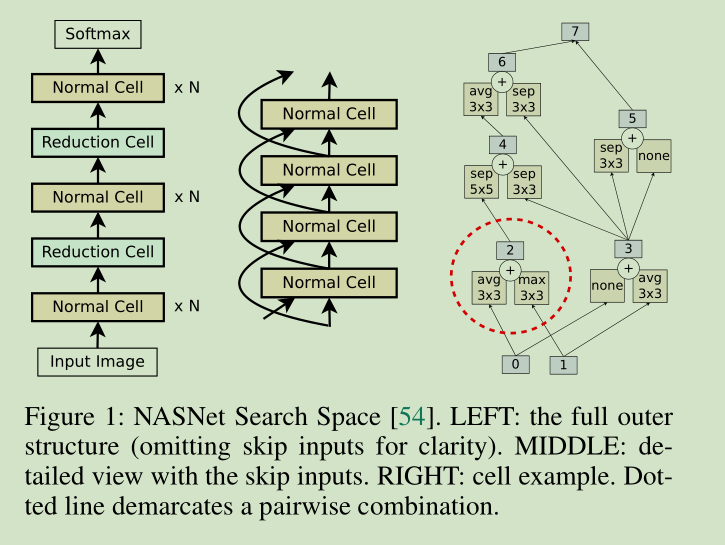
\includegraphics[width=0.4\textwidth]{figures/architecture.png}
   \caption{The artitecture of a cell}\label{fig:digit}
   \label{f_artc}
  \end{figure}

  \subsection{Overall Neural Network Architecture}
  As is illustrated in Fig.\ref{total_artc} overall network consists of input layer, 6 identical cells, 3 polling layers, 2 fully connected perceptron layers, a softmax layer and an output layer. 

  \begin{figure}[H]
 	\centering
 	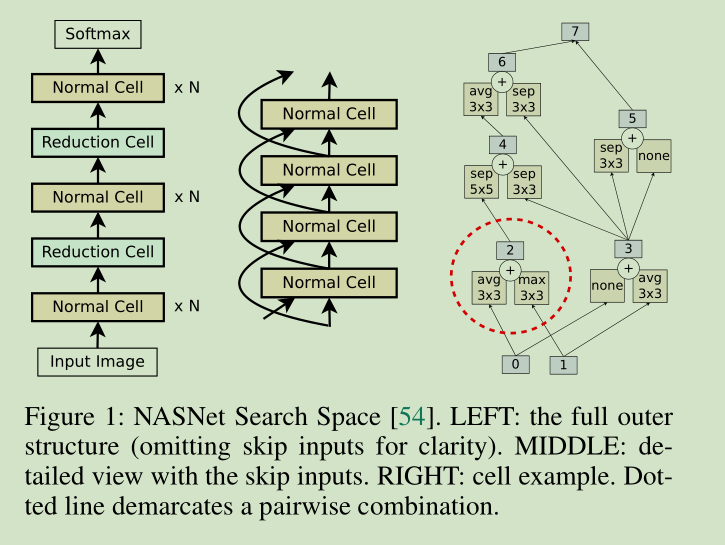
\includegraphics[width=0.4\textwidth]{figures/architecture.png}
   \caption{The overall artitecture of the total network. LEFT: outer structure. RIGHT: detailed skip connection of cells.}\label{fig:digit}
   \label{total_artc}
  \end{figure}

  For simplicity, all cells are the same. 
  \subsection{Evolutionary Algorithm Framework}
  For now, we follow the design of a cell based evolutionary NAS algorithm described in\cite{DBLP:journals/corr/abs-1802-01548} except that we propose a population update policy to preserve good parents. We will further examine initilization, crossover and mutation strategies to optimize our algorithm. We will also compare different performance estimation approaches to cut computation demand.

  \begin{algorithm}[htb]  
    \caption{ Elite Parent Preserving Evolution:}
    \begin{algorithmic}[1]  
  
    \State $population\gets \phi$
    \State $entireGen\gets \phi$
    \State $generation\gets 0$
    
    \While{$population$ size$<N$}
    \State $newNetwork\gets networkInit()$
    \State $trainNetwork(newNetwork)$
    \State add $newNetwork$ to $popution$ and $entireGen$
    \EndWhile
    
  
    
    \While {$genetation < G$}
      \State $parent\gets$ select a parent from population using tournament selection 
      \State $child \gets mutate(parent)$
      \State $trainNetwork(child)$
      \State add $child$ to $popution$ and $entireGen$
      \If {accuracy of $child$ is better than $P\%$ individuals in population}
        \State extend the $lifetime$ of $parent$ by $t$
      \EndIf
      
      \ForAll {$individual$ in $population$}
        \State update the $age$ of $individual$
        \State remove current $individual$ if its age reaches its $lifetime$
      \EndFor
      
      
    \EndWhile
    
    
    \\  
    \Return the network model with highest accuracy in $entireGen$
 
  \end{algorithmic}  
  \end{algorithm}  

The $population$ size is $N$ and the algorithm evolve $G$ generations in total. $entireGen$ stores all network models that we generated. 
     
In $networkInit()$, the initial network model is generated. Then its $age $ is set to 1 and $lifetime$ is set to the default value. 

$P$ and $t$ are hyper-parameters controlling the actual lifespan of an individual.




\section{--Proposed Framework}
 
  \begin{table}[H]
    
    \centering
      \begin{tabular}{cccc}
      \toprule
      Variable&Name\\
      \midrule
     
      $N_{total}$&size of the total population\\
  \bottomrule
  \end{tabular}
  \caption{Notation}
  \label{table:1}
  \end{table}

  \subsection{Fuzzy Rules}
  
  \begin{figure}[H]
 	\centering
 	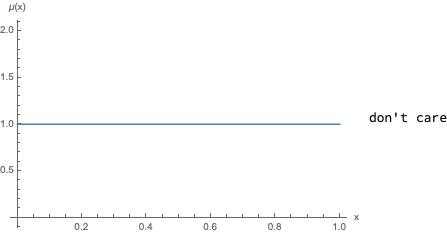
\includegraphics[width=0.4\textwidth]{figures/u1.png}
   \caption{The $don't care$ function}\label{fig:digit}
   \label{u0}
 \end{figure}
 \begin{figure}[H]
 	\centering
 	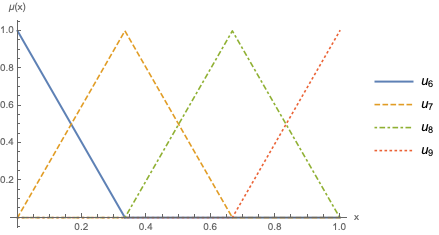
\includegraphics[width=0.4\textwidth]{figures/u4.png}
   \caption{Membership Functions with 4 intervals}\label{fig:digit}
   \label{u3}
 \end{figure}
  The antecedent part of $R_q$ is a set of antecedent fuzzy sets:
\begin{equation}A_q = \{A_{qi}|i = 1,2,...,n\}\end{equation}

   
  \section{Asynchronous Parallel Distributed System Design}
  
  \begin{figure}[H]
    \centering
    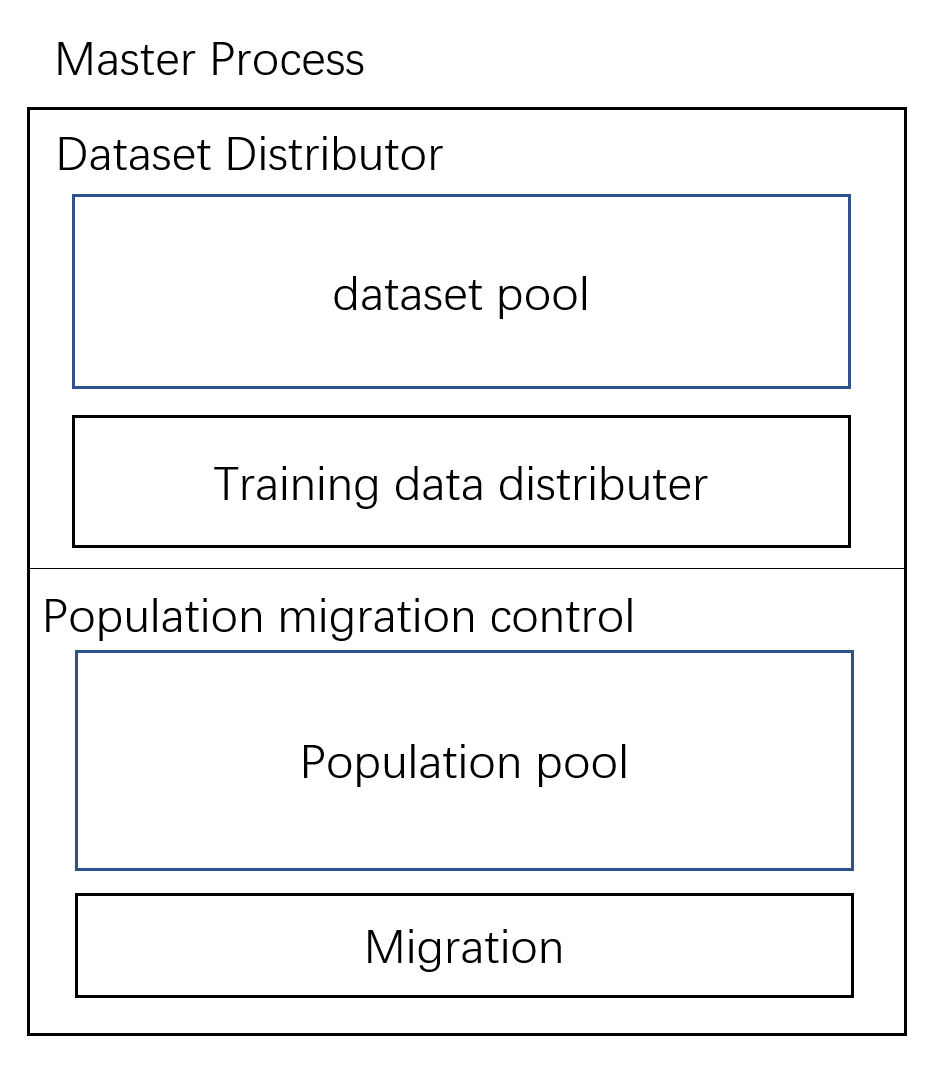
\includegraphics[width = 0.4\textwidth]{figures/master.png}
    \caption{The master process}
    \label{fig:master}
  \end{figure}

  \begin{figure}[H]
    \centering
    \includegraphics[width = 0.4\textwidth]{figures/slave.png}
    \caption{The slave process}
    \label{fig:slave}
  \end{figure}
  
  \subsection{Master and Slave process}
  \subsubsection{Master Process}
  
  \subsubsection{Slave Processes}\mbox{}
  
	\subsection{Dataset Distributor:}
	
  \subsection{Population Migration Control:}
  
	
  \subsection{Asynchronous Population Migration}
  
  
  \section{Experiments}

  \subsection{Pareto Front}
  \subsubsection{With different cores}
As is shown by Fig.\ref{diffCoreTr} and Fig.\ref{diffCoreT} ($I_{update} = 100, N_{total} = 264$), our model is able to get results that is similar to non-parallel models. Note that with the increase of the number of cores, the ability of the model to obtain classifiers with more rules and antecedent fuzzy sets is decreasing, due to the decrease of sub-population. It's acceptable since our objective is to minimize the two objectives.
  \begin{figure}[H]
    \centering
    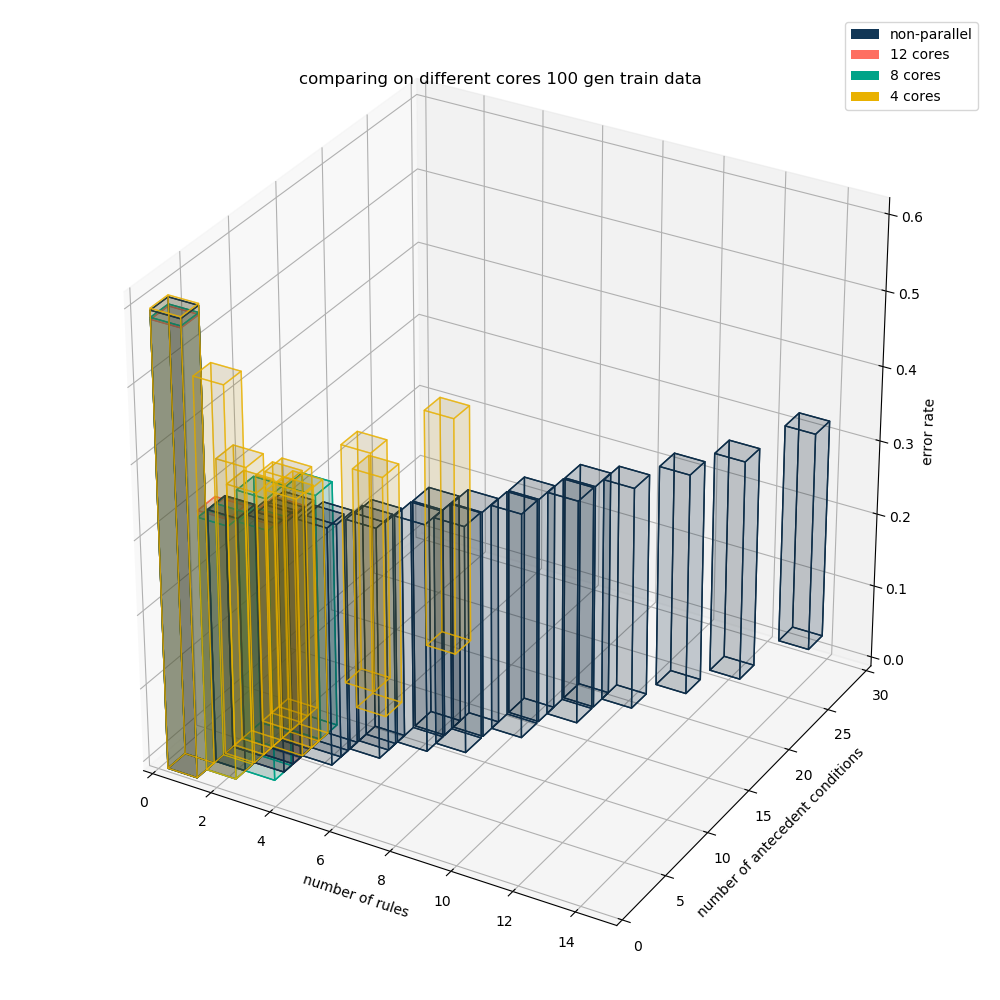
\includegraphics[width=0.38\textwidth]{figures/diffCoreTrain.png}
    \caption{Pareto Front on training data}\label{diffCoreTr}
  \end{figure}
  \begin{figure}[H]
    \centering
    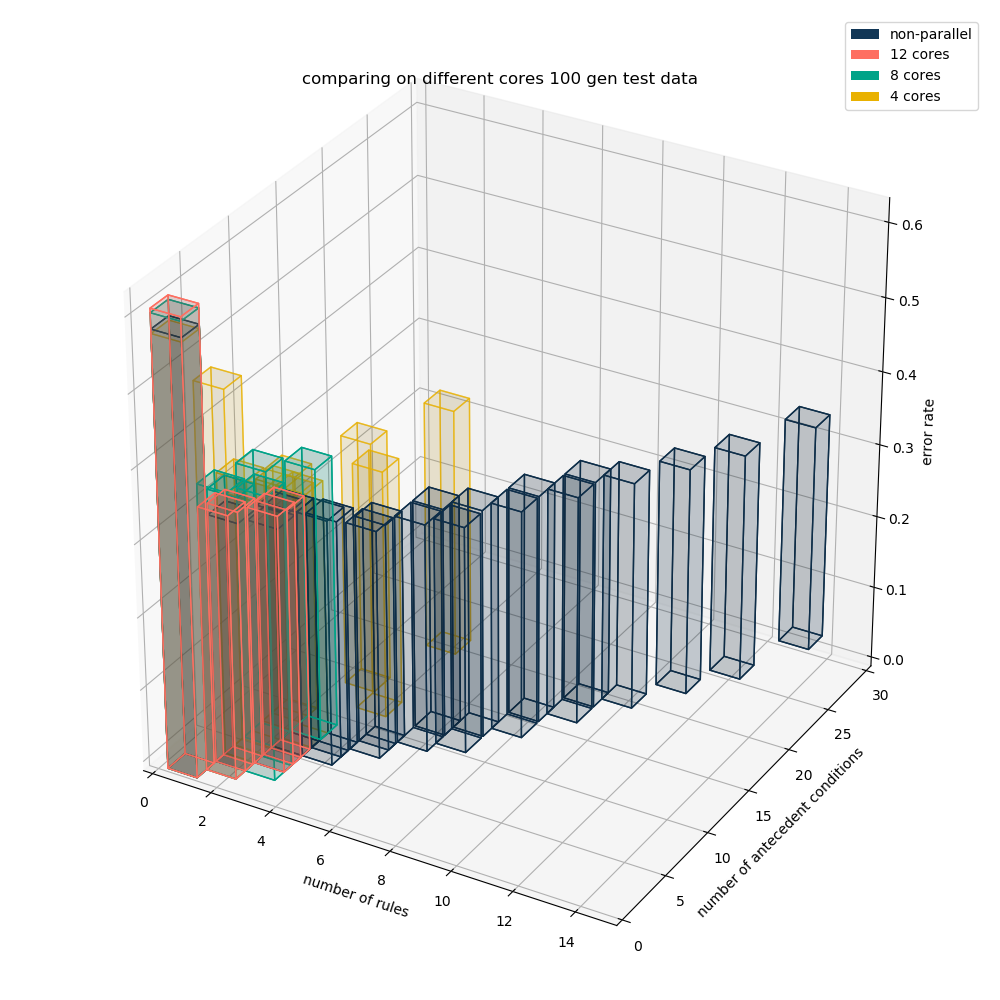
\includegraphics[width=0.38\textwidth]{figures/diffCoreTest.png}
    \caption{Pareto Front on test data}\label{diffCoreT}
  \end{figure}
  
  
  
  \subsubsection{With different exchange interval}
  We can see from Fig.\ref{diffGenTr}, Fig.\ref{diffGenT} and Fig.\ref{diffTimeGen} ($N_{total} = 264, N_{island} = 8$) that the choice of exchange interval also impacts the performance of our model. A longer exchange interval leads to less communication between master and slave processes, thus reduces running time. 
  \begin{figure}[H]
    \centering
    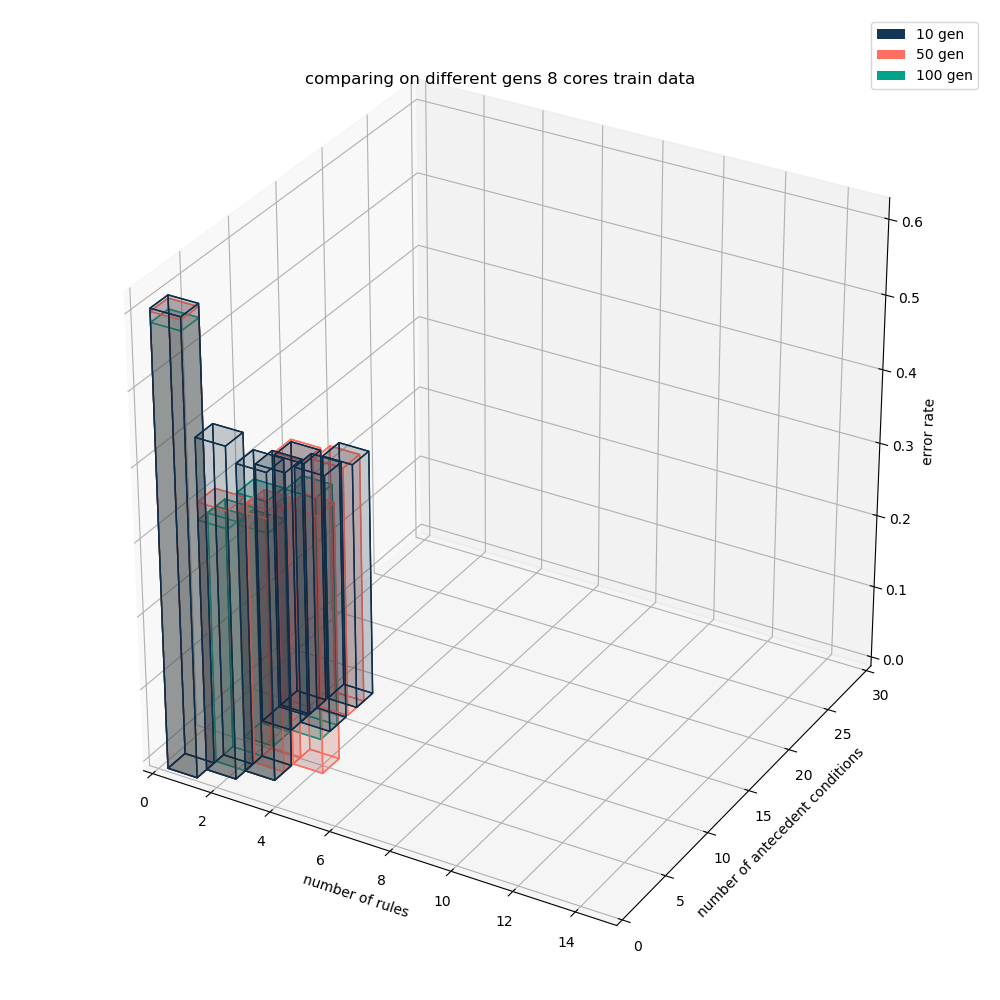
\includegraphics[width=0.4\textwidth]{figures/diffGenTrain.png}
    \caption{Pareto Front on training data with different $I_{update}$}\label{diffGenTr}
  \end{figure}
  \begin{figure}[H]
    \centering
    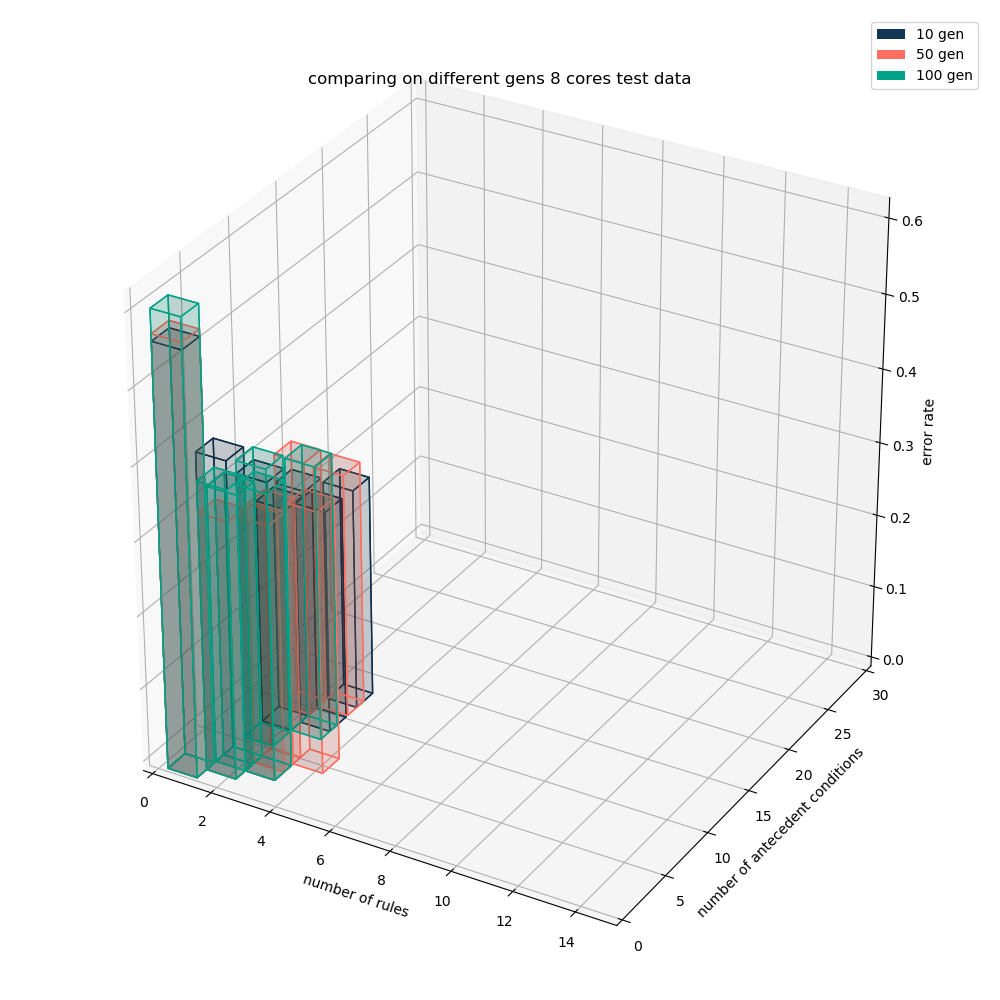
\includegraphics[width=0.4\textwidth]{figures/diffGenTest.png}
    \caption{Pareto Front on training data with different $I_{update}$}\label{diffGenT}
  \end{figure}

  \begin{figure}[H]
    \centering
    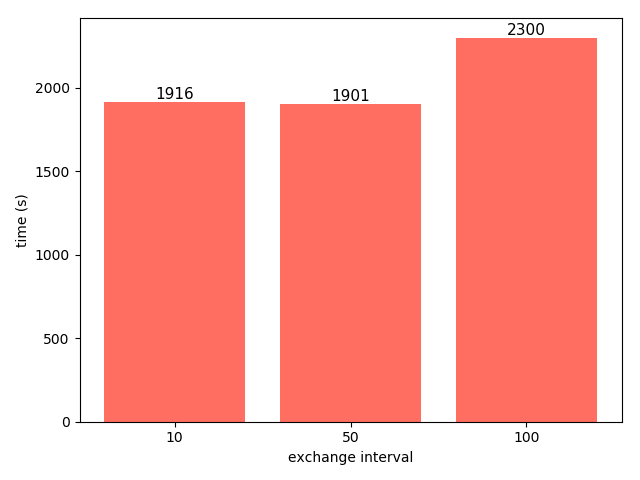
\includegraphics[width=0.4\textwidth]{figures/diffTimeGen.png}
    \caption{Computational time with different $I_{update}$}\label{diffTimeGen}
  \end{figure}



\subsection{Computation Time}
\begin{figure}[H]
  \centering
  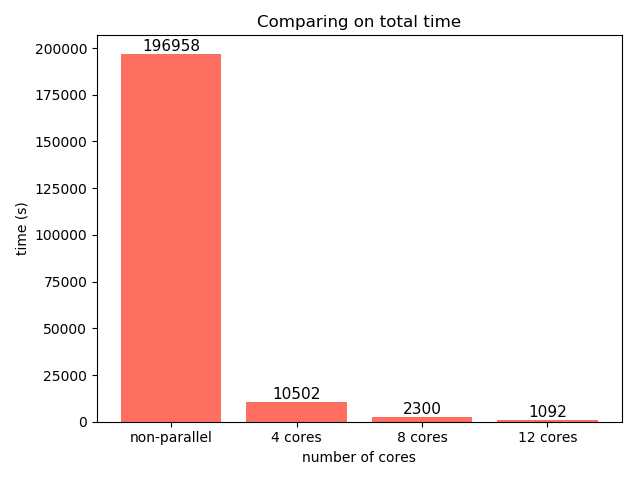
\includegraphics[width=0.4\textwidth]{figures/diffTime.png}
  \caption{Computation time of 3000 generations, $N_{pop}$ = 264.}\label{phT}
\end{figure}
With $n$ cores, we observe a speed up of up to $n^2$ times in our computational experiments.

\subsection{Compare with other model}
We compared our model with the synchronized model by Nojima et al.\cite{nojima2015application}, as is shown in Fig.\ref{diffModelTr}, Fig.\ref{diffModelTest} and Fig.\ref{diffModelTime}. The experiments are done using 8 cores.

\begin{figure}[H]
  \centering
  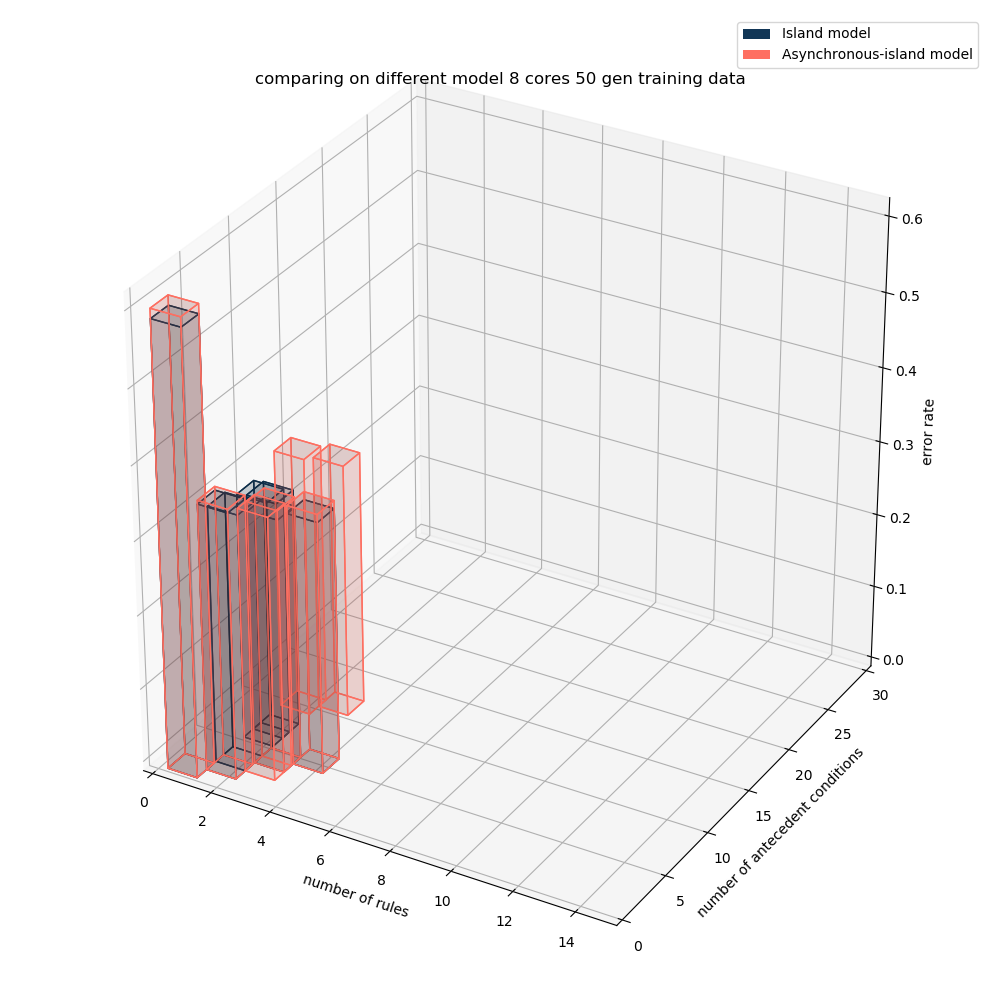
\includegraphics[width=0.4\textwidth]{figures/diffModelTrain.png}
  \caption{Comparison on training data.}\label{diffModelTr}
\end{figure}
\begin{figure}[H]
  \centering
  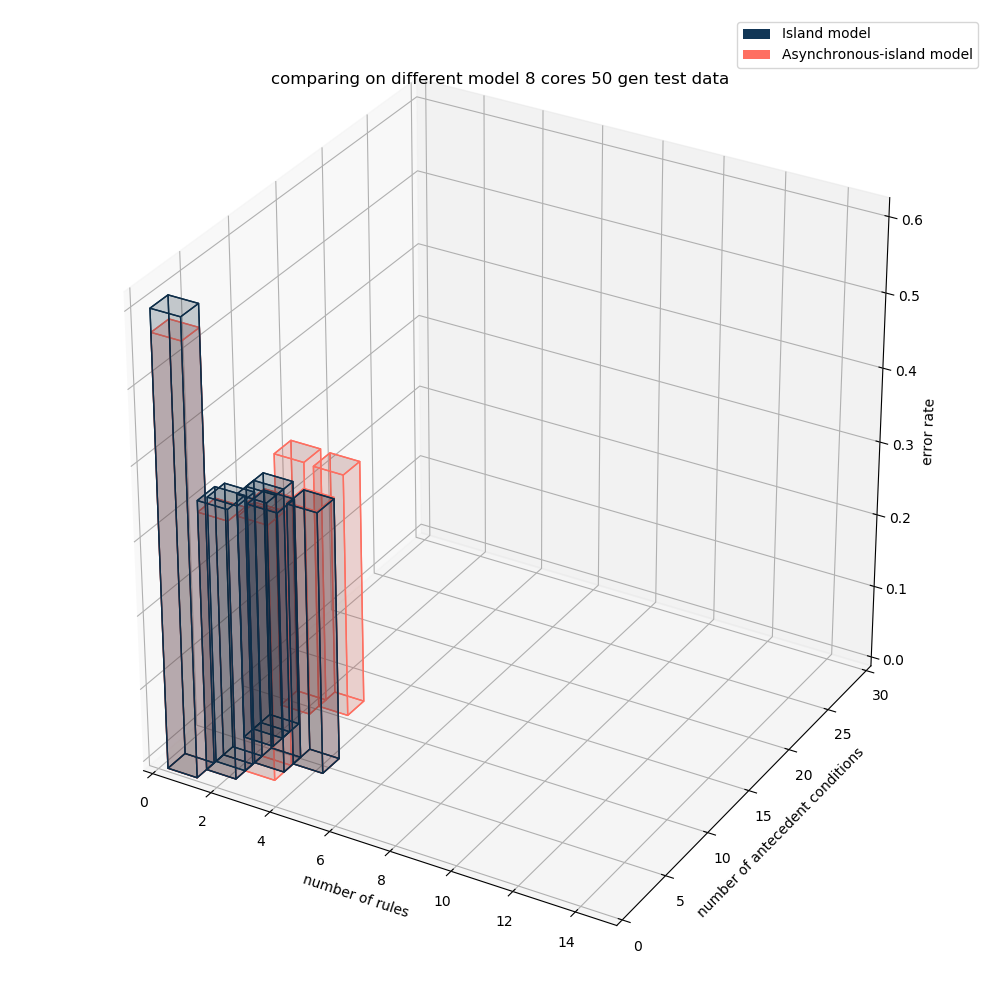
\includegraphics[width=0.4\textwidth]{figures/diffModelTest.png}
  \caption{Comparison on test data.}\label{diffModelTest}
\end{figure}
\begin{figure}[H]
  \centering
  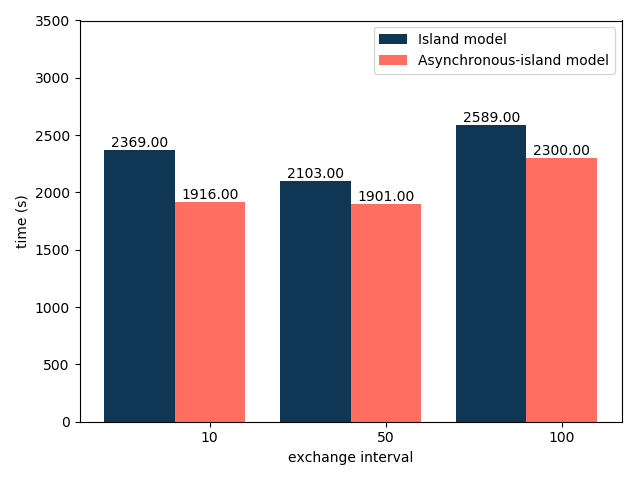
\includegraphics[width=0.4\textwidth]{figures/diffModelTime.png}
  \caption{Comparison on total time.}\label{diffModelTime}
\end{figure}


 \section{Conclusion}
 
  \section{Contribution}
  
   

\bibliographystyle{ieeetr}
\bibliography{ref}
% that's all folks
\end{document}


  